\chapter{Termodinámica estadística aplicada}\label{ch:b3:statistical-thermo-applied}

El hidrógeno líquido guardado en el depósito mejor aislado sigue evaporándose y, en los
primeros días tras la licuefacción, se evapora mucho más deprisa de lo que explica el calor
que se filtra a través de las paredes. El calor procede del interior del líquido. Las moléculas de
hidrógeno existen en dos formas, que solo difieren en la orientación relativa de
los espines de sus dos protones y que se convierten una en otra muy
lentamente; a \qty{20}{K}, la conversión de una forma en la otra libera más
calor del necesario para evaporar el líquido. Este capítulo aplica las
funciones de partición del \cref{ch:b3:partition-functions} a las capacidades caloríficas, a
estos isómeros de espín nuclear y a la entropía que algunos cristales conservan a 0 K,
y calcula después constantes de equilibrio y efectos isotópicos solo a partir de datos
espectroscópicos.

\begin{recall}
El \cref{ch:b3:partition-functions} construyó la \omterm{def:b3:partition-functions:partition-function}{función de partición molecular} y sus
cuatro factores, y dedujo de ella $U$, $S$ y $G$. El volumen del segundo año relacionó
la constante de equilibrio estándar con la energía de Gibbs estándar de reacción,
$\Delta_rG^\circ = -RT\ln K^\circ$, y estableció la ecuación de van 't Hoff;
el \cref{ch:b3:many-electron-atoms} enunció que una función de onda cambia de signo cuando se intercambian dos
fermiones idénticos; el \cref{ch:b3:rovibrational-spectroscopy} encontró
la alternancia 3:1 de las intensidades de las rayas en el espectro Raman de rotación de las moléculas
del tipo de \ce{H2}. La parte del año 9 del primer volumen definió los isótopos.
\end{recall}

\begin{omfigure}
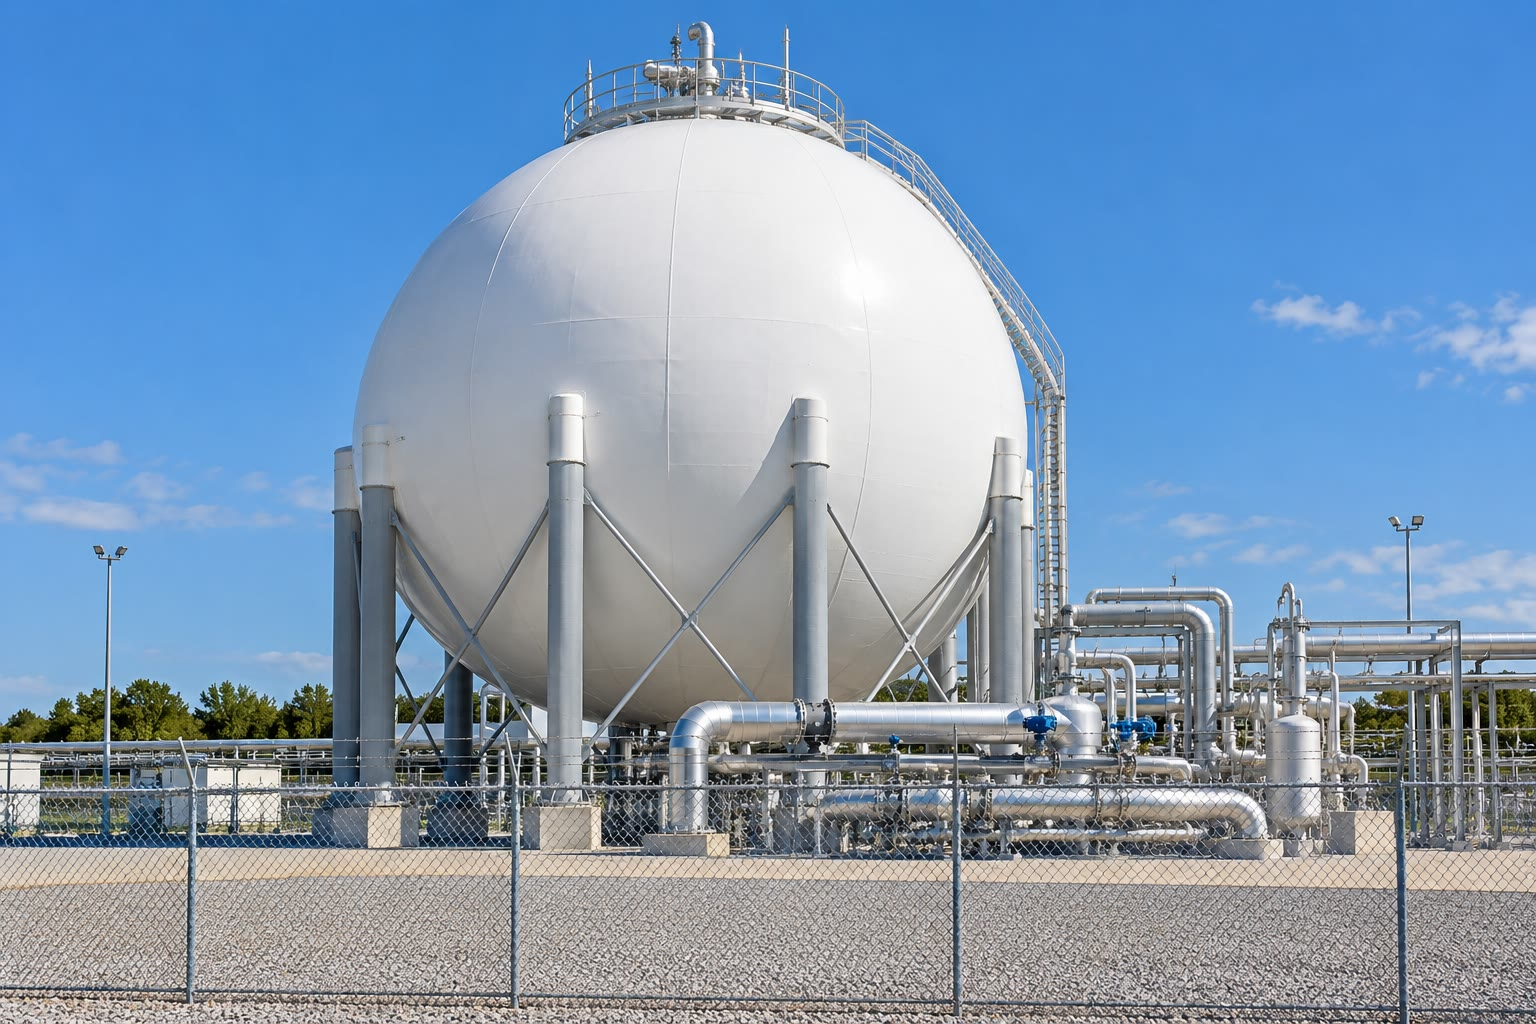
\includegraphics[width=0.6\linewidth]{images/book4/ai/b3-11-lh2-tank.jpg}

{\small Un depósito esférico de hidrógeno líquido. A \qty{20}{K}, el calor producido dentro del
líquido por la lenta conversión de una forma de espín nuclear del hidrógeno en la
otra puede superar al calor que se filtra desde el exterior.}
\end{omfigure}

\section{Capacidades caloríficas de los gases}

La capacidad calorífica a volumen constante es $C_V = (\partial U/\partial T)_V$, y con el
\cref{thm:b3:partition-functions:internal-energy} cada tipo de movimiento
contribuye por separado. Dos límites lo gobiernan todo.

\begin{theorem}[Teorema de equipartición]\label{thm:b3:statistical-thermo-applied:equipartition}
Cuando los niveles de energía de un movimiento están muy próximos en comparación con $kT$, cada
término de su energía que es cuadrático en una coordenada o en un momento contribuye con
$\frac12kT$ a la energía media de una molécula, y por tanto con $\frac12R$ a la capacidad
calorífica molar. Este enunciado es el \emph{teorema de equipartición}\index{teorema de equiparticion@teorema de equipartición}.
\end{theorem}

\begin{proof}[Demostración parcial]
En el límite clásico, la suma sobre los estados de un movimiento se convierte en una
integral, y un término cuadrático $a u^2$ aporta el factor $\int\eu^{-\beta au^2}\dd u =
\sqrt{\pi/\beta a}$, proporcional a $\beta^{-1/2}$. Por el
\cref{thm:b3:partition-functions:internal-energy}, su energía media es
$-\partial\ln(\beta^{-1/2})/\partial\beta = 1/2\beta = \frac12kT$. Que la integral clásica sea el
límite de la suma cuántica se demostró para la traslación y la rotación en el
\cref{ch:b3:partition-functions}; para la vibración se deduce de la proposición
siguiente cuando $T \gg \theta_{\mathrm V}$.
\end{proof}

La traslación tiene tres términos cuadráticos ($\frac32R$); la rotación de una molécula
lineal, dos ($R$), y la de una no lineal, tres ($\frac32R$); cada vibración, dos,
cinético y potencial ($R$). Una molécula lineal de $N$ átomos tiende así a
$C_{V,\mathrm m} = \frac52R + (3N - 5)R$ a alta temperatura. Para las vibraciones, ese límite casi nunca
se alcanza a temperatura ambiente.

\begin{proposition}[Capacidad calorífica de vibración]\label{prop:b3:statistical-thermo-applied:cv-vib}
Una vibración armónica de temperatura característica $\theta_{\mathrm V}$ contribuye, con
$x = \theta_{\mathrm V}/T$,
\[
  \frac{C_{V,\mathrm m}^{\mathrm V}}{R} = \frac{x^2\eu^x}{(\eu^x - 1)^2},
\]
la función de Einstein, que tiende a 1 cuando $T \gg \theta_{\mathrm V}$ y disminuye
exponencialmente, como $x^2\eu^{-x}$, cuando $T \ll \theta_{\mathrm V}$.
\end{proposition}

\begin{proof}
A partir de la \cref{prop:b3:partition-functions:q-vib}, $U - U(0) = R\theta_{\mathrm V}/(\eu^x - 1)$ por mol.
Derivando respecto de $T$, con $\dd x/\dd T = -x/T$, se obtiene
$R\theta_{\mathrm V}\eu^x(x/T)/(\eu^x - 1)^2 = Rx^2\eu^x/(\eu^x - 1)^2$. Para $x \to 0$, $\eu^x - 1 \approx x$ y el
cociente tiende a 1; para $x$ grande se comporta como $x^2\eu^{-x}$.
\end{proof}

\begin{method}[La capacidad calorífica de un gas a partir de sus modos]\label{met:b3:statistical-thermo-applied:cv}
\begin{enumerate}
  \item Traslación: $\frac32R$, siempre.
  \item Rotación: $R$ (lineal) o $\frac32R$ (no lineal) si $T \gg \theta_{\mathrm R}$, lo que se cumple para todos los
        gases salvo el hidrógeno por encima de unas decenas de kelvin.
  \item Vibraciones: un término de Einstein por \omterm{def:b3:group-theory-applied:normal-mode}{modo normal}, con $\theta_{\mathrm V} = hc\tilde\nu/k$ a partir de
        los números de onda fundamentales; un modo degenerado cuenta tantas veces como
        su \omterm{def:b3:quantum-model-systems:degenerate}{degeneración}.
  \item Sumar, y $C_{p,\mathrm m} = C_{V,\mathrm m} + R$ para un gas ideal.
\end{enumerate}
\end{method}

Se dice que un movimiento está congelado cuando $kT$ es pequeño frente a su primera
excitación: entonces no almacena energía y no contribuye a $C_V$. La
vibración de \ce{N2} ($\theta_{\mathrm V} = \qty{3352}{K}$) está congelada a temperatura ambiente y
$C_{V,\mathrm m} = \frac52R$; la de \ce{Cl2} ($\theta_{\mathrm V} = \qty{798}{K}$) está medio despierta,
$C_{V,\mathrm m} = 3.07R$ a \qty{300}{K}.

\begin{omfigure}
\begin{tikzpicture}
\begin{axis}[width=0.86\linewidth, height=6.4cm, xmode=log, xmin=10, xmax=3000,
  ymin=1.3, ymax=3.9, axis lines=left, xlabel={$T$ / K}, ylabel={$C_{V,\mathrm m}/R$},
  tick label style={font=\small}, label style={font=\small},
  log ticks with fixed point, xtick={10,30,100,300,1000,3000},
  unbounded coords=jump]
\addplot[omDef, thick] table[x=T, y=N2] {figdata/out/bachelor-3-heat-capacity.dat};
\addplot[black!60, thick] table[x=T, y=Cl2] {figdata/out/bachelor-3-heat-capacity.dat};
\addplot[omThm, thick, dashed] table[x=T, y=nH2] {figdata/out/bachelor-3-heat-capacity.dat};
\addplot[omThm, thick] table[x=T, y=eH2] {figdata/out/bachelor-3-heat-capacity.dat};
\addplot[only marks, mark=*, mark size=1.6pt, omDef] table[x=T, y=N2] {figdata/out/bachelor-3-heat-capacity-janaf.dat};
\addplot[only marks, mark=square*, mark size=1.5pt, black!60] table[x=T, y=Cl2] {figdata/out/bachelor-3-heat-capacity-janaf.dat};
\draw[black!30, densely dotted] (axis cs:10,1.5) -- (axis cs:3000,1.5);
\draw[black!30, densely dotted] (axis cs:10,2.5) -- (axis cs:3000,2.5);
\draw[black!30, densely dotted] (axis cs:10,3.5) -- (axis cs:3000,3.5);
\node[font=\scriptsize, black!60, anchor=south east] at (axis cs:2900,1.5) {$\frac32$: traslación};
\node[font=\scriptsize, black!60, anchor=south west] at (axis cs:10.5,2.5) {$\frac52$: + rotación};
\node[font=\scriptsize, black!60, anchor=south west] at (axis cs:10.5,3.5) {$\frac72$: + vibración};
\node[font=\scriptsize, omThm, anchor=south west] at (axis cs:60,3.6) {\ce{H2} en equilibrio};
\node[font=\scriptsize, omThm, anchor=north west] at (axis cs:130,1.78) {\ce{H2} normal};
\node[font=\scriptsize, black!70, anchor=south east] at (axis cs:560,3.33) {\ce{Cl2}};
\node[font=\scriptsize, omDef, anchor=south east] at (axis cs:1000,3.0) {\ce{N2}};
\end{axis}
\end{tikzpicture}

{\small Capacidad calorífica molar a volumen constante, calculada a partir de las constantes
espectroscópicas (líneas; \omterm{def:b3:quantum-model-systems:rotor}{rotor rígido}, vibración armónica), con los valores de las
tablas termoquímicas para \ce{N2} y \ce{Cl2} (puntos, $C_p/R - 1$). La vibración se despierta
hacia $\theta_{\mathrm V}/10$; por encima de unos \qty{1000}{K}, las tablas superan al modelo armónico,
que no tiene en cuenta la anarmonicidad. Hidrógeno: la contribución de rotación
del hidrógeno normal (trazo discontinuo, orto y para congelados en 3:1) y del hidrógeno
en equilibrio (trazo continuo), que sobrepasa $\frac52$ porque convertir para en orto
absorbe calor.}
\end{omfigure}

\section{Estadística de espín nuclear}

Los dos núcleos de \ce{H2} son fermiones idénticos. Intercambiarlos cambia el signo
de la función de onda total (\cref{ch:b3:many-electron-atoms}); intercambiarlos es
lo mismo que dar la vuelta a la molécula de extremo a extremo, lo que multiplica la función de onda de
rotación $Y_{J,M}$ por $(-1)^J$ y la función de espín nuclear por $+1$ o $-1$.

\begin{theorem}[Estadística de espín nuclear]\label{thm:b3:statistical-thermo-applied:spin-statistics}
En una molécula diatómica homonuclear cuyos núcleos tienen espín $I$, en un estado
electrónico fundamental ${}^1\Sigma_g^+$, hay $(2I+1)(I+1)$ estados de espín nuclear simétricos y $(2I+1)I$
antisimétricos. Para los fermiones ($I$ semientero), los
antisimétricos van con $J$ par y los simétricos con $J$ impar; para los
bosones ($I$ entero), al revés. Para \ce{H2} ($I = \frac12$), los niveles pares e impares tienen
pesos de espín 1 y 3; para \ce{D2} ($I = 1$), 6 y 3. Cuando $I = 0$ solo existe una paridad de
$J$: la molécula lineal de \ce{CO2}, con dos núcleos \ce{^{16}O} y un
estado fundamental simétrico, solo tiene niveles de rotación pares.
\end{theorem}

\begin{proof}[Demostración parcial]
El postulado de simetrización (la función de onda total es antisimétrica frente al
intercambio de dos fermiones idénticos y simétrica para los bosones) se admite. Los
$(2I+1)^2$ productos de estados de espín de un núcleo $|m_1\rangle|m_2\rangle$ dan $2I+1$ estados
simétricos con $m_1 = m_2$ y, para cada uno de los $(2I+1)2I/2$ pares $m_1 \ne m_2$, una
combinación simétrica y una antisimétrica: $(2I+1) + (2I+1)I = (2I+1)(I+1)$
estados simétricos y $(2I+1)I$ antisimétricos. En un estado ${}^1\Sigma_g^+$, las funciones electrónica
y de vibración no cambian con el intercambio, de modo que el producto de las
funciones de rotación y de espín debe tener el signo global exigido: para los
fermiones, $(-1)^J \times(\text{simetría de espín}) = -1$, lo que empareja $J$ par con los
estados de espín antisimétricos. Para \ce{H2}: 3 simétricos, 1 antisimétrico; para \ce{D2}: 6 y
3.
\end{proof}

\begin{definition}[Ortohidrógeno y parahidrógeno]\label{def:b3:statistical-thermo-applied:spin-isomers}
El \emph{ortohidrógeno}\index{ortohidrogeno@ortohidrógeno} es la forma de \ce{H2} con los espines de los dos
protones en un estado simétrico (triplete), que solo ocupa los niveles de rotación
impares; el \emph{parahidrógeno}\index{parahidrogeno@parahidrógeno}, la forma con el
estado de espín antisimétrico (singlete), que solo ocupa los niveles pares.
\end{definition}

Convertir una en otra exige invertir un espín nuclear respecto del
otro, lo que las colisiones con otras moléculas de hidrógeno apenas consiguen: en el hidrógeno
puro, las dos formas se comportan durante días como dos gases distintos. Una superficie
paramagnética, cuyo campo magnético inhomogéneo actúa de forma distinta sobre los dos
protones, cataliza la conversión.

\begin{proposition}[Razón orto--para en el equilibrio]\label{prop:b3:statistical-thermo-applied:ortho-para}
En el equilibrio, la fracción de \omterm{def:b3:statistical-thermo-applied:spin-isomers}{parahidrógeno} es
\[
  x_{\mathrm{para}} = \frac{\sum_{J\,\mathrm{par}}(2J+1)\eu^{-\theta_{\mathrm R}J(J+1)/T}}
    {\sum_{J\,\mathrm{par}}(2J+1)\eu^{-\theta_{\mathrm R}J(J+1)/T} + 3\sum_{J\,\mathrm{impar}}(2J+1)\eu^{-\theta_{\mathrm R}J(J+1)/T}},
\]
que tiende a 1 a 0 K y a $\frac14$ a alta temperatura. Para \ce{D2}, la forma orto
($J$ par) tiende a 1 a 0 K y a $\frac23$ a alta temperatura.
\end{proposition}

\begin{proof}
Es la \omterm{def:b3:partition-functions:boltzmann}{distribución de Boltzmann} sobre todos los estados, con los pesos de espín del
\cref{thm:b3:statistical-thermo-applied:spin-statistics}. A 0 K solo está poblado $J = 0$, que es
par. A alta temperatura, las sumas par e impar valen cada una la mitad
de $T/\theta_{\mathrm R}$, y la razón es $1 : 3$; para \ce{D2}, $6 : 3$.
\end{proof}

Para \ce{H2}, $\theta_{\mathrm R} = \qty{85.4}{K}$: la mezcla en equilibrio es mitad para a \qty{78}{K},
para en un 99.8\,\% en el punto de ebullición, \qty{20.37}{K}, y en un 25.07\,\% a temperatura
ambiente. El hidrógeno conservado a temperatura ambiente, llamado hidrógeno normal, es
por tanto una mezcla 3:1 de orto y para.

\begin{omfigure}
\begin{tikzpicture}
\begin{axis}[width=0.72\linewidth, height=5.4cm, xmin=0, xmax=300, ymin=0, ymax=1.05,
  axis lines=left, xlabel={$T$ / K}, ylabel={fracción en el equilibrio},
  tick label style={font=\small}, label style={font=\small}]
\addplot[omThm, thick] table[x=T, y=pH2] {figdata/out/bachelor-3-ortho-para.dat};
\addplot[omDef, thick] table[x=T, y=oD2] {figdata/out/bachelor-3-ortho-para.dat};
\draw[black!35, densely dotted] (axis cs:0,0.25) -- (axis cs:300,0.25);
\draw[black!35, densely dotted] (axis cs:0,0.6667) -- (axis cs:300,0.6667);
\node[font=\scriptsize, omThm, anchor=south west] at (axis cs:190,0.27) {fracción para de \ce{H2} $\to \frac14$};
\node[font=\scriptsize, omDef, anchor=south west] at (axis cs:120,0.69) {fracción orto de \ce{D2} $\to \frac23$};
\end{axis}
\end{tikzpicture}

{\small Composición en el equilibrio de los isómeros de espín nuclear en función de la
temperatura, a partir de los niveles de rotación y de los pesos de espín (\ce{H2}: 1 y 3;
\ce{D2}: 6 y 3). Las dos formas con $J$ par se imponen a baja temperatura.}
\end{omfigure}

La capacidad calorífica del hidrógeno muestra las consecuencias. En el hidrógeno normal, las
moléculas orto y para son dos gases mezclados en proporciones fijas; cada uno tiene su
propia escalera de niveles, que empieza en $J = 1$ y en $J = 0$, y su rotación se congela
por separado. En el hidrógeno en equilibrio, el calentamiento convierte además para en orto, lo que
absorbe energía y da el pico de la figura anterior. Las primeras medidas,
hechas sin catalizador, seguían la curva del hidrógeno normal, y fue la
interpretación de esa curva como una mezcla 3:1 congelada la que reveló por primera vez las
dos formas.

\begin{remark}
El \omterm{def:b3:partition-functions:symmetry-number}{número de simetría} de la \cref{prop:b3:partition-functions:q-rot} queda ahora justificado.
A alta temperatura, cada estado de espín encuentra permitidos alrededor de la mitad de los niveles de rotación,
de modo que $\sum(\text{peso de espín})(2J+1)\eu^{\dots} \approx (2I+1)^2\,T/2\theta_{\mathrm R}$: el
factor de espín total $(2I+1)^2$ se deja fuera por convenio, y queda $\sigma = 2$.
\end{remark}

\begin{definition}[Entropía residual]\label{def:b3:statistical-thermo-applied:residual-entropy}
La \emph{entropía residual}\index{entropia residual@entropía residual} de un cristal es la entropía que
conserva cuando $T \to 0$ porque sus moléculas quedan congeladas en una de muchas
disposiciones de energía igual o casi igual.
\end{definition}

\begin{proposition}[Entropías residuales del monóxido de carbono y del hielo]\label{prop:b3:statistical-thermo-applied:residual}
Un cristal de $N$ moléculas congelado en $W_0$ disposiciones igualmente probables tiene $S_0 =
k\ln W_0$. El \ce{CO} sólido, con cada molécula orientada en uno u otro sentido, tiene $S_{0,\mathrm m} = R\ln2 =
\qty{5.76}{J.K^{-1}.mol^{-1}}$. El hielo, con cada oxígeno enlazado a dos átomos de hidrógeno
y unido por enlaces de hidrógeno a otros dos, tiene $W_0 = (3/2)^N$ y $S_{0,\mathrm m} = R\ln\frac32 =
\qty{3.37}{J.K^{-1}.mol^{-1}}$.
\end{proposition}

\begin{proof}
La \cref{def:b3:partition-functions:statistical-entropy} aplicada para $T \to 0$.
\ce{CO}: el dipolo de la molécula es tan pequeño que las orientaciones CO y OC
tienen casi la misma energía, y cada una de las $N$ moléculas tiene dos: $W_0 = 2^N$,
$S_0 = Nk\ln2$. Hielo (recuento de Pauling): cada uno de los $2N$ átomos de hidrógeno está sobre una
línea O$\cdots$O, cerca de uno u otro extremo: $2^{2N}$ disposiciones. De las 16 maneras de
situar los cuatro hidrógenos en torno a un oxígeno, 6 le dan exactamente dos hidrógenos
próximos (una molécula de agua); tratando los oxígenos como independientes, una fracción
$6/16$ de las disposiciones satisface cada uno de ellos: $W_0 = 2^{2N}(6/16)^N = (3/2)^N$.
\end{proof}

Las tablas dan, para el \ce{CO}, la \omterm{def:b3:partition-functions:statistical-entropy}{entropía estadística}
(\cref{ch:b3:partition-functions}); el valor calorimétrico es más bajo en una diferencia del
orden de $R\ln2$, algo menor porque las orientaciones no son del todo
aleatorias. Para el hielo, la diferencia entre la entropía calorimétrica del vapor de agua y
su valor estadístico concordó con el recuento de Pauling cuando este lo hizo en 1935,
lo que confirmó que los protones del hielo están desordenados. El tercer principio,
en la forma ``la entropía de un cristal perfecto es nula a 0 K'', se aplica a los
cristales que alcanzan de verdad una sola disposición.

\begin{omfigure}
\begin{tikzpicture}[scale=1.15, every node/.style={transform shape}]
  \draw[black!45, dashed] (0.00,0.00) -- (1.20,0.00);
  \draw[black, thick] (0.00,0.00) -- (0.36,0.00); \node[aH, minimum size=2.2mm] at (0.36,0.00) {};
  \draw[black!45, dashed] (0.00,0.00) -- (0.00,1.20);
  \draw[black, thick] (0.00,0.00) -- (0.00,0.36); \node[aH, minimum size=2.2mm] at (0.00,0.36) {};
  \draw[black!45, dashed] (0.00,1.20) -- (1.20,1.20);
  \draw[black, thick] (0.00,1.20) -- (0.36,1.20); \node[aH, minimum size=2.2mm] at (0.36,1.20) {};
  \draw[black!45, dashed] (0.00,1.20) -- (0.00,2.40);
  \draw[black, thick] (0.00,2.40) -- (0.00,2.04); \node[aH, minimum size=2.2mm] at (0.00,2.04) {};
  \draw[black!45, dashed] (0.00,2.40) -- (1.20,2.40);
  \draw[black, thick] (1.20,2.40) -- (0.84,2.40); \node[aH, minimum size=2.2mm] at (0.84,2.40) {};
  \draw[black!45, dashed] (0.00,2.40) -- (0.00,3.60);
  \draw[black, thick] (0.00,3.60) -- (0.00,3.24); \node[aH, minimum size=2.2mm] at (0.00,3.24) {};
  \draw[black!45, dashed] (0.00,3.60) -- (1.20,3.60);
  \draw[black, thick] (1.20,3.60) -- (0.84,3.60); \node[aH, minimum size=2.2mm] at (0.84,3.60) {};
  \draw[black!45, dashed] (0.00,3.60) -- (0.00,4.20);
  \draw[black, thick] (0.00,3.60) -- (0.00,3.96); \node[aH, minimum size=2.2mm] at (0.00,3.96) {};
  \draw[black!45, dashed] (1.20,0.00) -- (2.40,0.00);
  \draw[black, thick] (1.20,0.00) -- (1.56,0.00); \node[aH, minimum size=2.2mm] at (1.56,0.00) {};
  \draw[black!45, dashed] (1.20,0.00) -- (1.20,1.20);
  \draw[black, thick] (1.20,1.20) -- (1.20,0.84); \node[aH, minimum size=2.2mm] at (1.20,0.84) {};
  \draw[black!45, dashed] (1.20,1.20) -- (2.40,1.20);
  \draw[black, thick] (2.40,1.20) -- (2.04,1.20); \node[aH, minimum size=2.2mm] at (2.04,1.20) {};
  \draw[black!45, dashed] (1.20,1.20) -- (1.20,2.40);
  \draw[black, thick] (1.20,1.20) -- (1.20,1.56); \node[aH, minimum size=2.2mm] at (1.20,1.56) {};
  \draw[black!45, dashed] (1.20,2.40) -- (2.40,2.40);
  \draw[black, thick] (1.20,2.40) -- (1.56,2.40); \node[aH, minimum size=2.2mm] at (1.56,2.40) {};
  \draw[black!45, dashed] (1.20,2.40) -- (1.20,3.60);
  \draw[black, thick] (1.20,3.60) -- (1.20,3.24); \node[aH, minimum size=2.2mm] at (1.20,3.24) {};
  \draw[black!45, dashed] (1.20,3.60) -- (2.40,3.60);
  \draw[black, thick] (2.40,3.60) -- (2.04,3.60); \node[aH, minimum size=2.2mm] at (2.04,3.60) {};
  \draw[black!45, dashed] (1.20,3.60) -- (1.20,4.20);
  \draw[black!45, dashed] (2.40,0.00) -- (3.60,0.00);
  \draw[black, thick] (3.60,0.00) -- (3.24,0.00); \node[aH, minimum size=2.2mm] at (3.24,0.00) {};
  \draw[black!45, dashed] (2.40,0.00) -- (2.40,1.20);
  \draw[black, thick] (2.40,0.00) -- (2.40,0.36); \node[aH, minimum size=2.2mm] at (2.40,0.36) {};
  \draw[black!45, dashed] (2.40,1.20) -- (3.60,1.20);
  \draw[black, thick] (2.40,1.20) -- (2.76,1.20); \node[aH, minimum size=2.2mm] at (2.76,1.20) {};
  \draw[black!45, dashed] (2.40,1.20) -- (2.40,2.40);
  \draw[black, thick] (2.40,2.40) -- (2.40,2.04); \node[aH, minimum size=2.2mm] at (2.40,2.04) {};
  \draw[black!45, dashed] (2.40,2.40) -- (3.60,2.40);
  \draw[black, thick] (3.60,2.40) -- (3.24,2.40); \node[aH, minimum size=2.2mm] at (3.24,2.40) {};
  \draw[black!45, dashed] (2.40,2.40) -- (2.40,3.60);
  \draw[black, thick] (2.40,2.40) -- (2.40,2.76); \node[aH, minimum size=2.2mm] at (2.40,2.76) {};
  \draw[black!45, dashed] (2.40,3.60) -- (3.60,3.60);
  \draw[black, thick] (2.40,3.60) -- (2.76,3.60); \node[aH, minimum size=2.2mm] at (2.76,3.60) {};
  \draw[black!45, dashed] (2.40,3.60) -- (2.40,4.20);
  \draw[black!45, dashed] (3.60,0.00) -- (4.20,0.00);
  \draw[black, thick] (3.60,0.00) -- (3.96,0.00); \node[aH, minimum size=2.2mm] at (3.96,0.00) {};
  \draw[black!45, dashed] (3.60,0.00) -- (3.60,1.20);
  \draw[black, thick] (3.60,1.20) -- (3.60,0.84); \node[aH, minimum size=2.2mm] at (3.60,0.84) {};
  \draw[black!45, dashed] (3.60,1.20) -- (4.20,1.20);
  \draw[black!45, dashed] (3.60,1.20) -- (3.60,2.40);
  \draw[black, thick] (3.60,1.20) -- (3.60,1.56); \node[aH, minimum size=2.2mm] at (3.60,1.56) {};
  \draw[black!45, dashed] (3.60,2.40) -- (4.20,2.40);
  \draw[black!45, dashed] (3.60,2.40) -- (3.60,3.60);
  \draw[black, thick] (3.60,2.40) -- (3.60,2.76); \node[aH, minimum size=2.2mm] at (3.60,2.76) {};
  \draw[black!45, dashed] (3.60,3.60) -- (4.20,3.60);
  \draw[black, thick] (3.60,3.60) -- (3.96,3.60); \node[aH, minimum size=2.2mm] at (3.96,3.60) {};
  \draw[black!45, dashed] (3.60,3.60) -- (3.60,4.20);
  \draw[black, thick] (3.60,3.60) -- (3.60,3.96); \node[aH, minimum size=2.2mm] at (3.60,3.96) {};
  \draw[black!45, dashed] (-0.60,0.00) -- (0.00,0.00);
  \draw[black!45, dashed] (-0.60,1.20) -- (0.00,1.20);
  \draw[black, thick] (0.00,1.20) -- (-0.36,1.20); \node[aH, minimum size=2.2mm] at (-0.36,1.20) {};
  \draw[black!45, dashed] (-0.60,2.40) -- (0.00,2.40);
  \draw[black, thick] (0.00,2.40) -- (-0.36,2.40); \node[aH, minimum size=2.2mm] at (-0.36,2.40) {};
  \draw[black!45, dashed] (-0.60,3.60) -- (0.00,3.60);
  \draw[black!45, dashed] (0.00,-0.60) -- (0.00,0.00);
  \draw[black!45, dashed] (1.20,-0.60) -- (1.20,0.00);
  \draw[black, thick] (1.20,0.00) -- (1.20,-0.36); \node[aH, minimum size=2.2mm] at (1.20,-0.36) {};
  \draw[black!45, dashed] (2.40,-0.60) -- (2.40,0.00);
  \draw[black, thick] (2.40,0.00) -- (2.40,-0.36); \node[aH, minimum size=2.2mm] at (2.40,-0.36) {};
  \draw[black!45, dashed] (3.60,-0.60) -- (3.60,0.00);
  \node[aO, minimum size=4mm] at (0.00,0.00) {};
  \node[aO, minimum size=4mm] at (0.00,1.20) {};
  \node[aO, minimum size=4mm] at (0.00,2.40) {};
  \node[aO, minimum size=4mm] at (0.00,3.60) {};
  \node[aO, minimum size=4mm] at (1.20,0.00) {};
  \node[aO, minimum size=4mm] at (1.20,1.20) {};
  \node[aO, minimum size=4mm] at (1.20,2.40) {};
  \node[aO, minimum size=4mm] at (1.20,3.60) {};
  \node[aO, minimum size=4mm] at (2.40,0.00) {};
  \node[aO, minimum size=4mm] at (2.40,1.20) {};
  \node[aO, minimum size=4mm] at (2.40,2.40) {};
  \node[aO, minimum size=4mm] at (2.40,3.60) {};
  \node[aO, minimum size=4mm] at (3.60,0.00) {};
  \node[aO, minimum size=4mm] at (3.60,1.20) {};
  \node[aO, minimum size=4mm] at (3.60,2.40) {};
  \node[aO, minimum size=4mm] at (3.60,3.60) {};
\end{tikzpicture}

{\small El desorden de los protones en el hielo, dibujado como una red cuadrada plana (la red
real es tetraédrica): cada oxígeno (rojo) tiene cuatro vecinos O$\cdots$O, un
hidrógeno (blanco) en cada línea, y exactamente dos hidrógenos próximos a él (las reglas
del hielo). Es una de las $(3/2)^N$ disposiciones del recuento de Pauling; todas
tienen casi la misma energía, y la congelación elige una al azar.}
\end{omfigure}

\section{Constantes de equilibrio a partir de las funciones de partición}

\begin{theorem}[Constante de equilibrio a partir de las funciones de partición]\label{thm:b3:statistical-thermo-applied:k-from-q}
Para una reacción $0 = \sum_J\nu_J\mathrm J$ entre gases ideales,
\[
  K^\circ = \prod_J\Bigl(\frac{q^\circ_{J,\mathrm m}}{N_A}\Bigr)^{\nu_J}\eu^{-\Delta_rE_0/RT},
\]
donde $q^\circ_{J,\mathrm m}$ es la función de partición de $\mathrm J$ en el volumen molar estándar
$V^\circ_{\mathrm m} = RT/p^\circ$, cada una contada desde su propio estado fundamental, y $\Delta_rE_0 =
\sum\nu_JE_{0,J}$ es la energía molar de reacción a 0 K, desde el estado fundamental de
los reactivos hasta el de los productos.
\end{theorem}

\begin{proof}
Según el \cref{thm:b3:partition-functions:entropy}, un mol de gas ideal $\mathrm J$ a $p^\circ$ tiene la energía de Gibbs
$G^\circ_{\mathrm m} - G_{\mathrm m}(0) = -RT\ln(q^\circ_{J,\mathrm m}/N_A)$, y $G_{\mathrm m}(0)$ es la energía $E_{0,J}$
de su estado fundamental en una escala común a todas las especies. Así, $\Delta_rG^\circ =
\Delta_rE_0 - RT\sum_J\nu_J\ln(q^\circ_{J,\mathrm m}/N_A)$, y $\Delta_rG^\circ = -RT\ln K^\circ$ da el
resultado.
\end{proof}

\begin{method}[Calcular una constante de equilibrio a partir de datos espectroscópicos]\label{met:b3:statistical-thermo-applied:k-stat}
\begin{enumerate}
  \item Para cada especie: $q^\circ_{\mathrm m}/N_A = (kT/p^\circ)\Lambda^{-3}\times q^{\mathrm R}q^{\mathrm V}q^{\mathrm E}$, con los
        \omterm{def:b3:partition-functions:symmetry-number}{números de simetría} y las \omterm{def:b3:quantum-model-systems:degenerate}{degeneraciones} electrónicas.
  \item $\Delta_rE_0$ a partir de las energías de disociación $D_0$ (medidas desde el nivel de vibración
        fundamental, de modo que incluyen las \omterm{def:b3:quantum-model-systems:oscillator}{energías de punto cero}) o de las
        entalpías de formación a 0 K.
  \item Multiplicar y comprobar las unidades: $K^\circ$ es un número puro, y la presión
        estándar entra a través de $kT/p^\circ$.
\end{enumerate}
\end{method}

\begin{example}[La disociación del yodo]\label{ex:b3:statistical-thermo-applied:iodine}
% ledger: janaf:I.dfH0, janaf:I2g.dfH0, lev:I.2P1_2, diat:I2.we, diat:I2.wexe, diat:I2.Be, diat:I2.ae, aw:I, janaf:I.logKf.1000
Para $\ce{I2(g) <=> 2 I(g)}$, $\Delta_rE_0 = D_0(\ce{I2}) = 2 \times 107.164 - 65.504 = \qty{148.824}{kJ/mol}$
a partir de las entalpías de formación a 0 K de las tablas termoquímicas. A
\qty{1000}{K}: para I, $\Lambda = \qty{4.90}{pm}$, $kT/p^\circ = \qty{1.381e-25}{m^3}$, $q^{\mathrm E} = 4 +
2\eu^{-10.94} = 4.0000$ (el nivel ${}^2P_{1/2}$ está \qty{7603}{cm^{-1}} más arriba), luego $q^\circ_{\mathrm m}/N_A = \num{4.69e9}$;
para \ce{I2}, $\Lambda = \qty{3.47}{pm}$, $q^{\mathrm R} = 1000/(2 \times 0.05369) = 9313$ y $q^{\mathrm V} = 3.784$, luego
$q^\circ_{\mathrm m}/N_A = \num{1.17e14}$. Entonces $K^\circ = (4.69\times10^9)^2/(1.17\times10^{14}) \times \eu^{-17.90} =
\num{3.17e-3}$, $\log K^\circ = -2.50$; las tablas dan $-2.51$.
\end{example}

\begin{omfigure}
\begin{tikzpicture}
\begin{axis}[name=ki, width=0.5\linewidth, height=5.6cm, xmin=0.58, xmax=1.45, ymin=-6.5,
  ymax=1, axis lines=left, xlabel={$1000\,\mathrm K/T$}, ylabel={$\log K^\circ$},
  tick label style={font=\small}, label style={font=\small},
  title={\small $\ce{I2 <=> 2 I}$}]
\addplot[black, thick] table[x=invT, y=logK] {figdata/out/bachelor-3-equilibrium-constant-stat-i2.dat};
\addplot[only marks, mark=*, mark size=1.8pt, omThm] table[x=invT, y=logK] {figdata/out/bachelor-3-equilibrium-constant-stat-i2-janaf.dat};
\node[font=\scriptsize, anchor=north east, align=right] at (axis cs:1.43,0.8) {línea: estadística\\ puntos: tablas};
\end{axis}
\begin{axis}[at={(ki.east)}, anchor=west, xshift=1.4cm, width=0.44\linewidth, height=5.6cm,
  xmin=0, xmax=2000, ymin=0, ymax=4.4, axis lines=left, xlabel={$T$ / K},
  ylabel={$K^\circ$}, tick label style={font=\small}, label style={font=\small},
  title={\small $\ce{H2 + D2 <=> 2 HD}$}, scaled x ticks=false,
  xticklabel style={/pgf/number format/1000 sep={}}]
\addplot[omDef, thick] table[x=T, y=K] {figdata/out/bachelor-3-equilibrium-constant-stat-hd.dat};
\draw[black!35, densely dotted] (axis cs:0,4) -- (axis cs:2000,4);
\node[font=\scriptsize, anchor=north east] at (axis cs:1950,3.95) {límite de $\sigma$: 4};
\end{axis}
\end{tikzpicture}

{\small Constantes de equilibrio calculadas a partir de las funciones de partición. Izquierda: la
disociación del yodo, una recta de van 't Hoff de pendiente $-\Delta_rH^\circ/(R\ln10)$, con
los valores de las tablas termoquímicas (puntos). Derecha: el intercambio $\ce{H2 + D2
<=> 2 HD}$, que tiende a la razón de los \omterm{def:b3:partition-functions:symmetry-number}{números de simetría}, 4, a alta temperatura
y queda por debajo a baja temperatura por las \omterm{def:b3:quantum-model-systems:oscillator}{energías de punto cero} y las
restricciones de espín nuclear.}
\end{omfigure}

\begin{proposition}[El intercambio H$_2$ + D$_2$]\label{prop:b3:statistical-thermo-applied:hd}
Para $\ce{H2 + D2 <=> 2 HD}$, $K^\circ \to 4$ a alta temperatura.
\end{proposition}

\begin{proof}
A alta temperatura, los factores de traslación, rotación y vibración son
$m^{3/2}$, $T/\sigma\theta_{\mathrm R} \propto \mu/\sigma$ y $T/\theta_{\mathrm V} \propto \sqrt\mu$ (la \omterm{def:b3:quantum-model-systems:oscillator}{constante de fuerza}, una
propiedad electrónica, es la misma para las tres moléculas), y $\Delta_rE_0/RT \to 0$.
Con $m_{\ce{H2}} = 2$, $m_{\ce{D2}} = 4$, $m_{\ce{HD}} = 3$ y $\mu = 1/2$, 1, $2/3$ (en unidades de la
masa del protón, despreciando la pequeña diferencia entre D y 2H):
\[
  K^\circ \to \Bigl(\frac{9}{8}\Bigr)^{3/2} \times \frac{(2/3)^2/1^2}{(1/2)(1)/(2 \times 2)}
  \times \frac{2/3}{\sqrt{1/2}\sqrt1}
  = \frac{27}{16\sqrt2} \times \frac{32}{9} \times \frac{2\sqrt2}{3} = 4 .
\]
Todos los factores de masa se cancelan exactamente, y solo quedan los \omterm{def:b3:partition-functions:symmetry-number}{números de
simetría}: $\sigma_{\ce{H2}}
\sigma_{\ce{D2}}/\sigma_{\ce{HD}}^2 = 4$.
\end{proof}

A \qty{298.15}{K}, la constante estadística vale 3.26: las \omterm{def:b3:quantum-model-systems:oscillator}{energías de punto cero} de \ce{H2},
\ce{D2} y HD (\qty{2170.3}{cm^{-1}}, \qty{1542.3}{cm^{-1}} y \qty{1883.7}{cm^{-1}}) dan $\Delta_rE_0 =
\qty{54.8}{cm^{-1}}$, un factor $\eu^{-54.8/207.2} = 0.77$; la rotación, aún parcialmente cuantizada en
estas moléculas ligeras, también cuenta.

\begin{proposition}[La ecuación de van 't Hoff, recuperada]\label{prop:b3:statistical-thermo-applied:vant-hoff-stat}
La constante de equilibrio estadística obedece a $\dfrac{\dd\ln K^\circ}{\dd T} = \dfrac{\Delta_rH^\circ}{RT^2}$.
\end{proposition}

\begin{proof}
Cada $q^\circ_{J,\mathrm m}$ depende de $T$ a través de sus niveles y a través de $V^\circ_{\mathrm m} = RT/p^\circ$:
$\dd\ln q^\circ_{J,\mathrm m}/\dd T = (U_J - U_J(0))/RT^2 + 1/T$ por mol, por el
\cref{thm:b3:partition-functions:internal-energy}. Por tanto, $\dd\ln K^\circ/\dd T =
[\Delta_rE_0 + \sum\nu_J(U_J - U_J(0)) + \sum\nu_JRT]/RT^2 = (\Delta_rU + \Delta\nu_{\mathrm g}RT)/RT^2 =
\Delta_rH^\circ/RT^2$ para gases ideales.
\end{proof}

De la pendiente del panel izquierdo de la figura se obtiene que la entalpía de disociación del
yodo hacia \qty{1000}{K} es \qty{154}{kJ/mol}: $D_0$ más la energía de traslación
adicional de dos átomos respecto de una molécula, menos su energía de rotación y de
vibración.

\section{Efectos isotópicos}

Los \omterm{def:b3:rovibrational-spectroscopy:rotational-constant}{isotopólogos} tienen la misma estructura electrónica, y por tanto la misma curva de energía
potencial y las mismas \omterm{def:b3:quantum-model-systems:oscillator}{constantes de fuerza}, pero masas distintas: sus números de onda de
vibración, sus \omterm{def:b3:quantum-model-systems:oscillator}{energías de punto cero} y sus funciones de partición difieren, y también
sus constantes de equilibrio.

\begin{definition}[Efecto isotópico de equilibrio, factor de fraccionamiento, valor $\delta$]\label{def:b3:statistical-thermo-applied:isotope-effect}
El \emph{efecto isotópico de equilibrio}\index{efecto isotopico de equilibrio@efecto isotópico de equilibrio} de una
reacción es la razón $K_{\mathrm{ligero}}/K_{\mathrm{pesado}}$ de sus constantes de equilibrio con el
isótopo ligero y con el pesado. El \emph{factor de fraccionamiento}\index{factor de fraccionamiento}
entre dos fases o compuestos A y B es $\alpha_{\mathrm{A/B}} = R_{\mathrm A}/R_{\mathrm B}$, donde
$R$ es la razón del isótopo pesado al ligero (por ejemplo, $\ce{^{18}O}/\ce{^{16}O}$). El
\emph{valor $\delta$}\index{valor delta@valor $\delta$} de una muestra es $\delta = (R_{\mathrm{muestra}}/R_{\text{patrón}}
- 1) \times 1000$, en tanto por mil (\textperthousand).
\end{definition}

\begin{proposition}[Efectos isotópicos a partir de las energías de punto cero]\label{prop:b3:statistical-thermo-applied:zpe-isotope}
Para un intercambio $\ce{XH + YD <=> XD + YH}$ a temperaturas a las que las vibraciones de
tensión están congeladas, el factor dominante de la constante de equilibrio es
\[
  K \approx \exp\Bigl(-\frac{\Delta\mathrm{ZPE}}{kT}\Bigr), \qquad
  \Delta\mathrm{ZPE} = \tfrac12hc\bigl[\tilde\nu_{\mathrm{XD}} + \tilde\nu_{\mathrm{YH}} - \tilde\nu_{\mathrm{XH}} - \tilde\nu_{\mathrm{YD}}\bigr],
\]
y $\tilde\nu_{\mathrm D} \approx \tilde\nu_{\mathrm H}/\sqrt2$ para un hidrógeno unido a un átomo pesado. El isótopo
pesado se concentra en el enlace más rígido.
\end{proposition}

\begin{proof}
El \cref{thm:b3:statistical-thermo-applied:k-from-q}, con las energías medidas
desde el fondo de las curvas de potencial comunes: $\Delta_rE_0$ es la variación de la
\omterm{def:b3:quantum-model-systems:oscillator}{energía de punto cero}. Los factores de traslación y de rotación casi se cancelan
entre dos intercambios de los mismos isótopos sobre compañeros pesados, y las
funciones de partición de vibración valen 1 cuando están congeladas. Con $\tilde\nu \propto \mu^{-1/2}$ y
$\mu_{\mathrm{XD}} \approx 2\mu_{\mathrm{XH}}$ para X pesado, $\tilde\nu_{\mathrm{XD}} = \tilde\nu_{\mathrm{XH}}/\sqrt2$, y $\Delta\mathrm{ZPE} =
\frac12hc(1 - 1/\sqrt2)(\tilde\nu_{\mathrm{YH}} - \tilde\nu_{\mathrm{XH}})$: negativa, luego $K > 1$, cuando X--H es el
enlace más rígido.
\end{proof}

El mismo razonamiento explica el fraccionamiento de los isótopos del oxígeno entre el agua
y su vapor, entre el agua y el carbonato de una concha, o entre dos
minerales: el \omterm{def:b3:statistical-thermo-applied:isotope-effect}{factor de fraccionamiento} tiende a 1 a alta temperatura (como
$K_{\mathrm{HD}}$ tiende a su límite de simetría) y se aleja de 1 al bajar la
temperatura. Medido como valores $\delta$, es un termómetro: el $\delta^{18}$O del carbonato
de las conchas fósiles registra la temperatura del agua en la que crecieron, y
el del hielo de los sondeos polares, la temperatura de las nubes que formaron su
nieve.

\begin{inthelab}[Un convertidor orto--para]
Un licuefactor de hidrógeno enfría el gas por etapas y, entre una etapa y otra, lo hace pasar
por lechos de un catalizador paramagnético, normalmente óxido de hierro(III) hidratado.
El calor de conversión se elimina entonces a cada temperatura mediante el refrigerador,
y el líquido que llega al depósito está próximo a su composición de equilibrio,
casi totalmente para. Sin catalizador, el calor de conversión se
liberaría en el depósito.
\end{inthelab}

\begin{safety}{\ghs[0.8cm]{GHS02}\ghs[0.8cm]{GHS04}}
% ledger: ghs:H2
Hidrógeno: un gas extremadamente inflamable, almacenado a presión o como líquido
criogénico. Forma mezclas explosivas con el aire en un intervalo muy amplio y arde
con una llama casi invisible; el líquido causa quemaduras por frío y su vapor
desplaza al aire.
\end{safety}

\begin{history}[Los dos hidrógenos, 1927--1929]
Werner Heisenberg y Friedrich Hund predijeron en 1927 que las moléculas de hidrógeno
debían existir en dos formas que difieren en sus espines nucleares, y David Dennison
mostró ese mismo año que la desconcertante capacidad calorífica del hidrógeno medida
por debajo de la temperatura ambiente era la de una mezcla 3:1 de ambas, congelada en su
composición de temperatura ambiente. En 1929, Karl Friedrich Bonhoeffer y Paul
Harteck adsorbieron hidrógeno sobre carbón a la temperatura del aire líquido, desorbieron
\omterm{def:b3:statistical-thermo-applied:spin-isomers}{parahidrógeno} casi puro, reconocible por su distinta conductividad térmica,
y comprobaron que solo volvía muy lentamente a la mezcla normal.
\end{history}

\section{Ejercicios}

\begin{exercise}[$\star$]\label{exo:b3:statistical-thermo-applied:1}
Dese el límite de alta temperatura de $C_{V,\mathrm m}$ del \ce{CO2} (lineal, 3 átomos), e indíquese
qué contribuciones siguen congeladas a temperatura ambiente.
\end{exercise}

\begin{exercise}[$\star$]\label{exo:b3:statistical-thermo-applied:2}
Evalúese la función de Einstein en $T = \theta_{\mathrm V}$ y en $T = \theta_{\mathrm V}/10$.
\end{exercise}

\begin{exercise}[$\star$]\label{exo:b3:statistical-thermo-applied:3}
% ledger: diat:H2.Be, diat:H2.ae
Con $\theta_{\mathrm R} = \qty{85.35}{K}$ para \ce{H2}, calcúlese la fracción de para en el equilibrio a
\qty{20}{K} (solo importan $J = 0$ y $J = 1$) y a \qty{77}{K} ($J \le 3$).
\end{exercise}

\begin{exercise}[$\star$]\label{exo:b3:statistical-thermo-applied:4}
Explíquese por qué el deuterio (espín nuclear 1) da pesos orto:para de $6 : 3$, qué
forma es la estable a 0 K y cuál es la razón a temperatura ambiente.
\end{exercise}

\begin{exercise}[$\star\star$]\label{exo:b3:statistical-thermo-applied:5}
% ledger: diat:H2.we, diat:H2.wexe, diat:D2.we, diat:D2.wexe, diat:HD.we, diat:HD.wexe
Las \omterm{def:b3:quantum-model-systems:oscillator}{energías de punto cero} de \ce{H2}, \ce{D2} y HD son 2170.3, 1542.3 y
\qty{1883.7}{cm^{-1}}. Calcúlense $\Delta_rE_0$ para $\ce{H2 + D2 <=> 2 HD}$ y el factor $\eu^{-\Delta_rE_0/RT}$ a
\qty{298.15}{K}. Compárese $4\eu^{-\Delta_rE_0/RT}$ con el valor estadístico completo, 3.26.
\end{exercise}

\begin{exercise}[$\star\star$]\label{exo:b3:statistical-thermo-applied:6}
Estímese la \omterm{def:b3:statistical-thermo-applied:residual-entropy}{entropía residual} de un cristal de \ce{N2O} (NNO lineal, que puede
orientarse en uno u otro sentido) y de \ce{CH3D} (que puede situar su D en cualquiera de cuatro
posiciones).
\end{exercise}

\begin{exercise}[$\star\star$]\label{exo:b3:statistical-thermo-applied:7}
% ledger: diat:Cl2.we, diat:Cl2.wexe, janaf:Cl2.Cp.300
Calcúlese la $C_{p,\mathrm m}$ de \ce{Cl2} a \qty{300}{K} a partir de $\theta_{\mathrm V} = \qty{797.6}{K}$ y compárese con el
valor tabulado, \qty{33.981}{J.K^{-1}.mol^{-1}}.
\end{exercise}

\begin{exercise}[$\star\star$]\label{exo:b3:statistical-thermo-applied:8}
% ledger: diat:I2.we, diat:I2.wexe
Calcúlese la capacidad calorífica de vibración de \ce{I2} ($\theta_{\mathrm V} = \qty{306.9}{K}$) a
\qty{298.15}{K}, como fracción de su valor de equipartición.
\end{exercise}

\begin{exercise}[$\star\star$]\label{exo:b3:statistical-thermo-applied:9}
Una muestra de agua A tiene $\delta^{18}\mathrm O = -10.0$\,\textperthousand\ y una muestra B,
$+2.0$\,\textperthousand\ en la misma escala. ¿Cuál es más rica en \ce{^{18}O}? Calcúlese el
\omterm{def:b3:statistical-thermo-applied:isotope-effect}{factor de fraccionamiento} $\alpha_{\mathrm{A/B}}$.
\end{exercise}

\begin{exercise}[$\star\star\star$]\label{exo:b3:statistical-thermo-applied:10}
En el intercambio $\ce{XH + YD <=> XD + YH}$ (datos del ejercicio), $\tilde\nu_{\mathrm{XH}} =
\qty{3000}{cm^{-1}}$ y $\tilde\nu_{\mathrm{YH}} = \qty{2000}{cm^{-1}}$, con X e Y pesados. Estímese $K$ a
\qty{298.15}{K} y dígase adónde va el deuterio.
\end{exercise}

\begin{exercise}[$\star\star\star$]\label{exo:b3:statistical-thermo-applied:11}
% ledger: janaf:I.dfH0, janaf:I2g.dfH0, lev:I.2P1_2, diat:I2.we, diat:I2.wexe, diat:I2.Be, diat:I2.ae, aw:I
Las constantes estadísticas de $\ce{I2 <=> 2 I}$ son $\log K^\circ = -3.392$ a \qty{900}{K} y
$-1.766$ a \qty{1100}{K}. Dedúzcase la $\Delta_rH^\circ$ media en el intervalo y explíquese
por qué supera a $D_0 = \qty{148.8}{kJ/mol}$.
\end{exercise}

\begin{exercise}[$\star\star\star$]\label{exo:b3:statistical-thermo-applied:12}
Para el \omterm{def:b3:statistical-thermo-applied:spin-isomers}{parahidrógeno} a baja temperatura solo importan $J = 0$ y $J = 2$. Demuéstrese que
su capacidad calorífica de rotación es $C/R = 5x^2\eu^{-x}/(1 + 5\eu^{-x})^2$ con $x = 6\theta_{\mathrm R}/T$, y
evalúese a \qty{100}{K} ($\theta_{\mathrm R} = \qty{85.35}{K}$).
\end{exercise}

\section{Problema: almacenar hidrógeno líquido}

\begin{problem}[{Problema de fin de semana --- almacenar hidrógeno líquido: las dos
formas de espín nuclear, el calor de su conversión, la evaporación que provoca y
el catalizador que la impide}]
\label{pb:b3:statistical-thermo-applied:1}
% ledger: diat:H2.Be, diat:H2.ae, diat:H2.De, hvap:nH2, tb:nH2, aw:H
El hidrógeno se licúa en su punto de ebullición, \qty{20.37}{K} a \qty{1.01325}{bar}, donde su
entalpía de vaporización es \qty{0.905}{kJ/mol}. Niveles de rotación: $F(J) = B_0J(J+1) -
D J^2(J+1)^2$ con $B_0 = \qty{59.322}{cm^{-1}}$ y $D = \qty{0.0471}{cm^{-1}}$ ($\theta_{\mathrm R} = \qty{85.35}{K}$).
Masa molar: \qty{2.016}{g/mol}. La conversión orto $\to$ para no catalizada en el líquido
se toma de primer orden, con $k = \qty{0.0114}{h^{-1}}$ (datos del problema).

\medskip\noindent\textbf{Parte I --- Las dos formas.}
\begin{enumerate}
  \item ¿Cuántos estados de espín nuclear tiene un par de protones? ¿Cuántos son
        simétricos frente al intercambio y cuántos antisimétricos?
  \item ¿Qué estados de espín van con $J$ par, cuáles con $J$ impar, y por qué?
  \item Dense los pesos de espín de los niveles pares e impares.
  \item Demuéstrese que la razón orto:para del hidrógeno a temperatura ambiente es 3:1.
  \item Calcúlese la energía de $J = 1$ por encima de $J = 0$, en \unit{cm^{-1}} y en
        \unit{kJ/mol}.
  \item Calcúlese la fracción de para en el equilibrio a \qty{20.37}{K}.
  \item La mezcla en equilibrio es mitad para hacia \qty{78}{K}. ¿Por qué esta
        temperatura está próxima a $\theta_{\mathrm R}$?
\end{enumerate}

\medskip\noindent\textbf{Parte II --- El calor de conversión.}
\begin{enumerate}[resume]
  \item ¿Cuál es la fracción de orto del hidrógeno recién licuado sin
        catalizador? ¿Por qué no cambia durante la licuefacción?
  \item Calcúlese el calor liberado cuando un mol de él alcanza el equilibrio a
        \qty{20.37}{K}.
  \item Exprésese por kilogramo.
  \item Exprésese la entalpía de vaporización por kilogramo.
  \item Compárense ambos.
  \item ¿Por qué un mejor aislamiento del depósito no puede eliminar este calor?
\end{enumerate}

\medskip\noindent\textbf{Parte III --- La evaporación.}
\begin{enumerate}[resume]
  \item Dese la fracción de orto tras un tiempo $t$ en el depósito.
  \item Calcúlese tras \qty{24}{h}.
  \item Calcúlese el calor liberado por mol de líquido en las primeras \qty{24}{h}.
  \item ¿Qué fracción del líquido evaporaría este calor?
  \item Repítase para una semana. ¿Por qué esta estimación sencilla exagera la pérdida?
  \item Calcúlese el periodo de semirreacción de la conversión.
\end{enumerate}

\medskip\noindent\textbf{Parte IV --- El catalizador y la capacidad calorífica.}
\begin{enumerate}[resume]
  \item ¿Dónde debe tener lugar la conversión en un licuefactor, y por qué?
  \item ¿Está el hidrógeno normal a \qty{300}{K} en equilibrio orto--para?
  \item ¿Por qué el hidrógeno normal y el hidrógeno en equilibrio tienen capacidades caloríficas distintas
        entre unos 30 y \qty{200}{K}?
  \item Léase en la figura de la capacidad calorífica el máximo de $C_{V,\mathrm m}/R$ del hidrógeno
        en equilibrio, y explíquese por qué supera $\frac52$.
  \item ¿Cuánto vale $C_{V,\mathrm m}/R$ del hidrógeno normal a \qty{50}{K}?
  \item Enúnciese el resultado: la razón entre el calor de conversión del hidrógeno normal
        y su entalpía de vaporización, y su significado para el depósito.
\end{enumerate}
\end{problem}
